\section{Simulation Analysis}\label{section:sim}

\subsection{Operating Point Analysis for t$<$0}

First of all, to contextualize the values obtained using the tools in ngspice, it is necessary to state that, as node 0 is connected to ground, its nodal voltage does not appear on the table of results. Furthermore, to be able to describe the voltage flowing in the dependent source, it is necessary to know the current in resistor 6. However, ngspice is not able to compute this value when the depedent source is described. So, in order to do that, an extra dependent voltage source (whose voltage drop is equal to 0 V) was created, and put in series after the resistor 6. This led to the appearence of node 8, that has the same voltage drop as node 6. So, by doing that, ngspice is able to determine the current in this auxiliar independent source, which is exactly the value needed.
 The circuit with these changes is shown in the drawing below.

\begin{figure}[ht] \centering
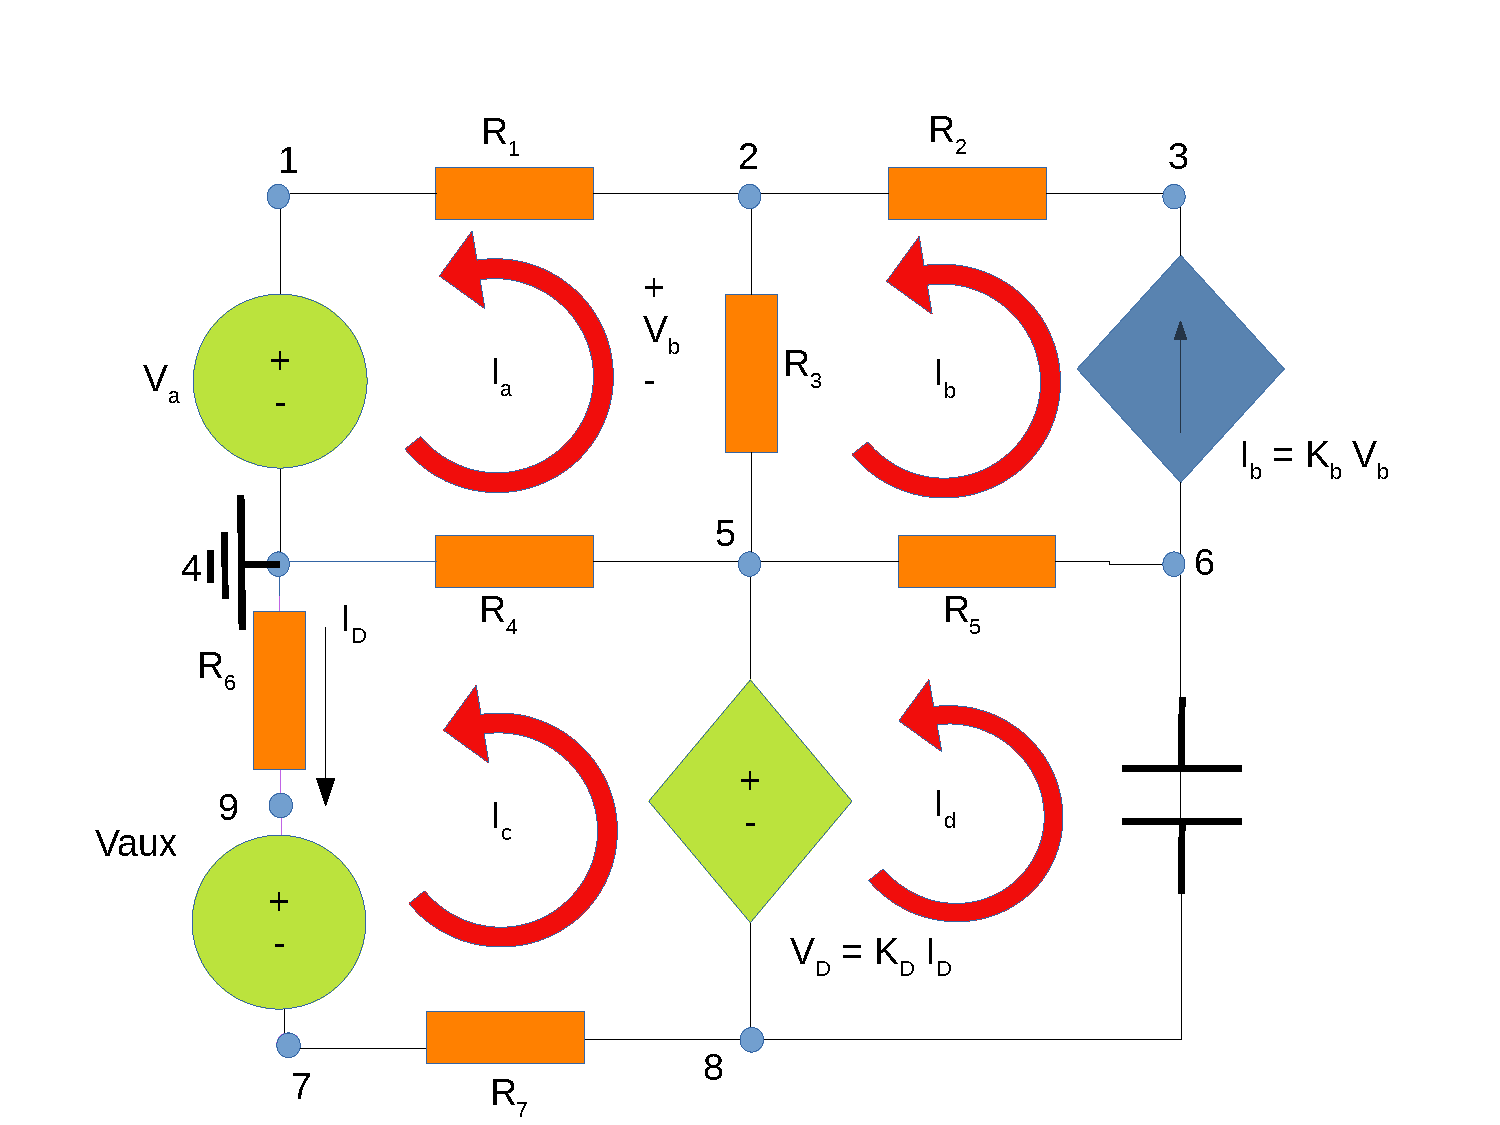
\includegraphics[width=0.8\linewidth]{sim1draw.pdf}
\caption{Circuit analysed in ngspice.}
\label{simdraw}
\end{figure}

\subsection{Operating Point Analysis}
As requested, an operating point analysis was conducted. The capacitor was replaced by the independent voltage source $V_{x}$ (\ref{sim2draw}). The values of currents and nodal voltages  were then put in a table, as well as the $R_{eq}$, hence:

\begin{equation}
R_{eq}=\frac{v(6)-v(8)}{vxbranch}
\label{eq:4}
\end{equation}


\subsection{Operating Point Analysis for $\ge$ 0 (Natural Solution)}


In this section, a transient analysis was made in order to evaluate the natural response of the circuit, which means, the variation over time. The description of the circuit included the initial values of v(6) and v(8), calculated in question 1. As the ngspice and octave results matched, as observed in \ref{subsection:2.3}, the theorectical values were imported from a .cir file created by octave.
The time interval considered was [0,20]ms.
\begin{figure}[h] \centering
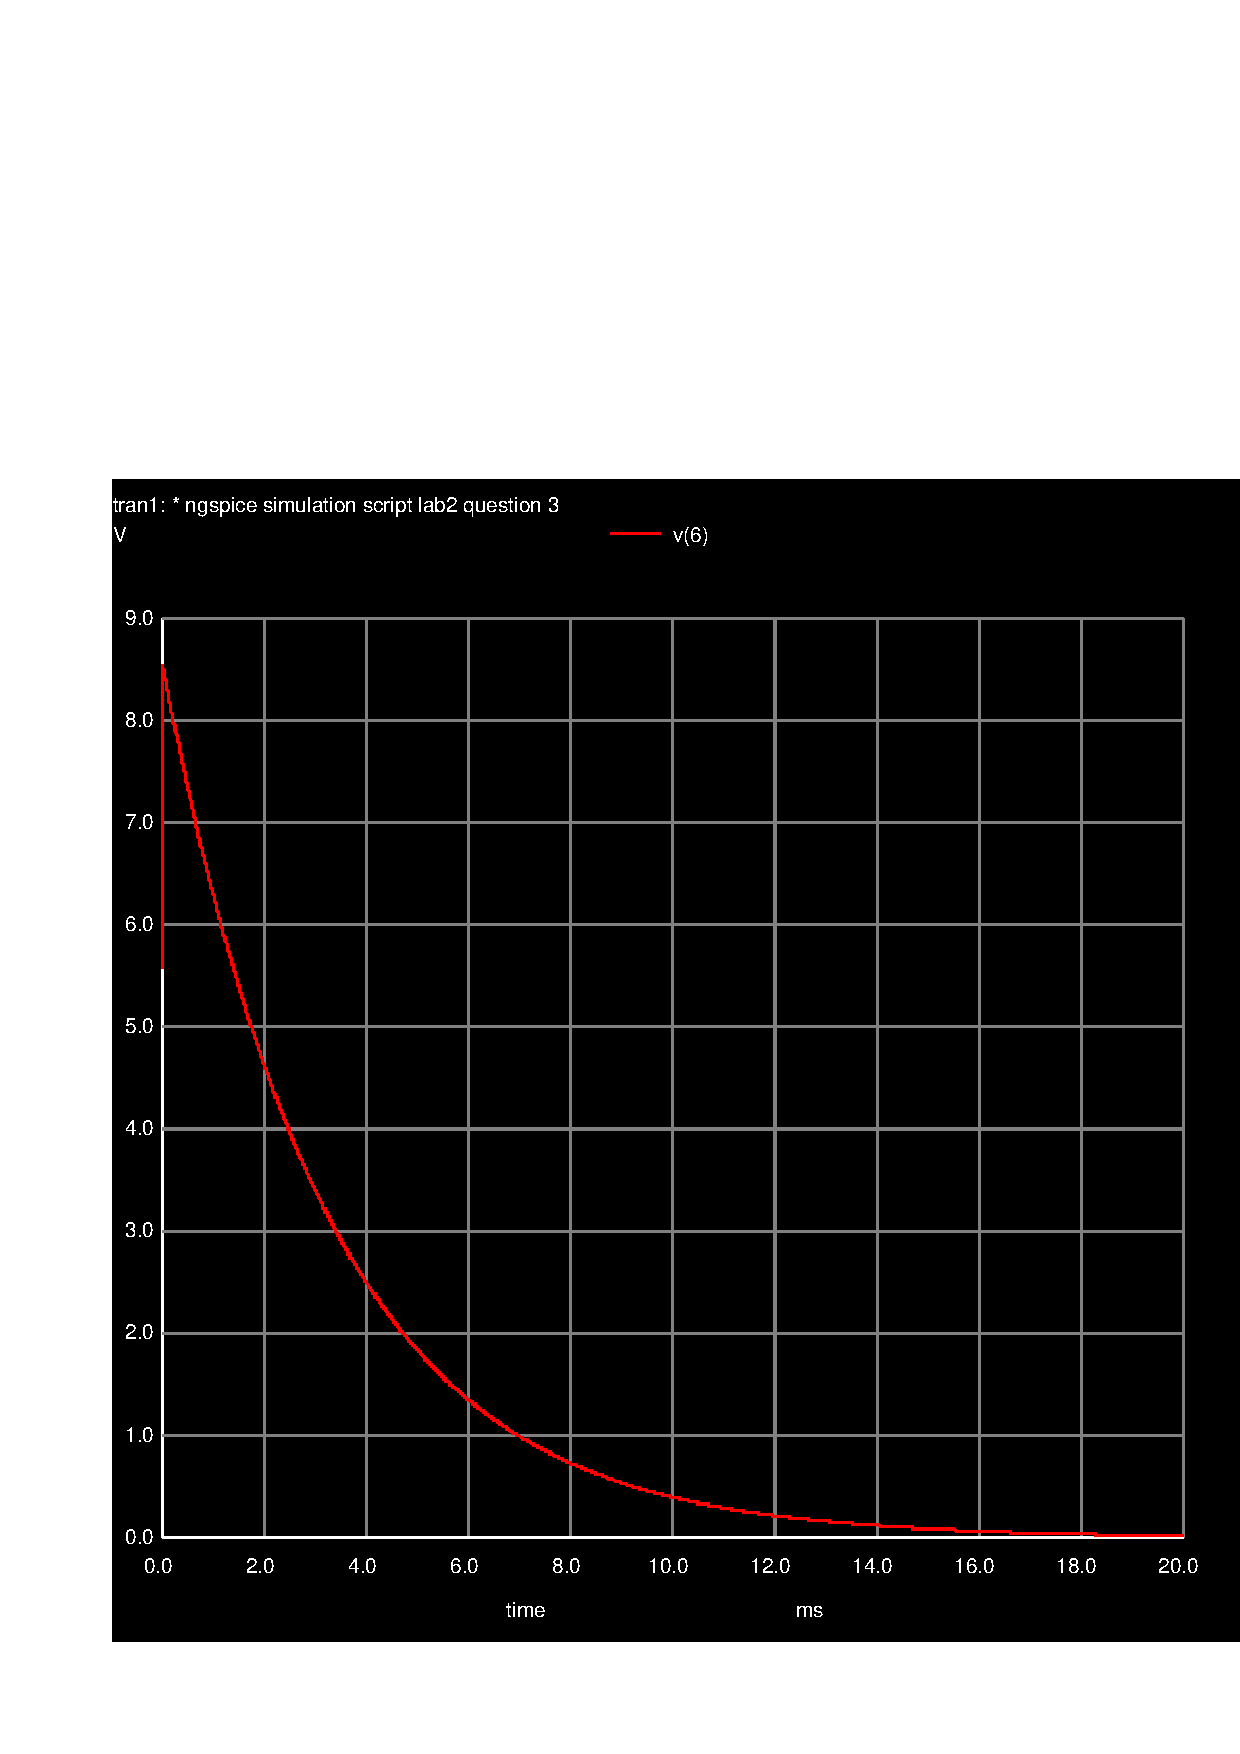
\includegraphics[width=0.5\linewidth]{sim3.pdf}
\caption{Circuit analysed.}
\label{fig:sim3}
\end{figure}
\newpage


\subsection{Operating Point Analysis for $\ge$ 0 (Natural and Forced Solutions)}

Once again, a transient analysis was made in order to meet the goal above. The main difference between the analysis in question 3 and this one is that Vs was considered a sinusoidal voltage source. This way, the plot obtained is the sum of both responses.

\begin{figure}[h] \centering
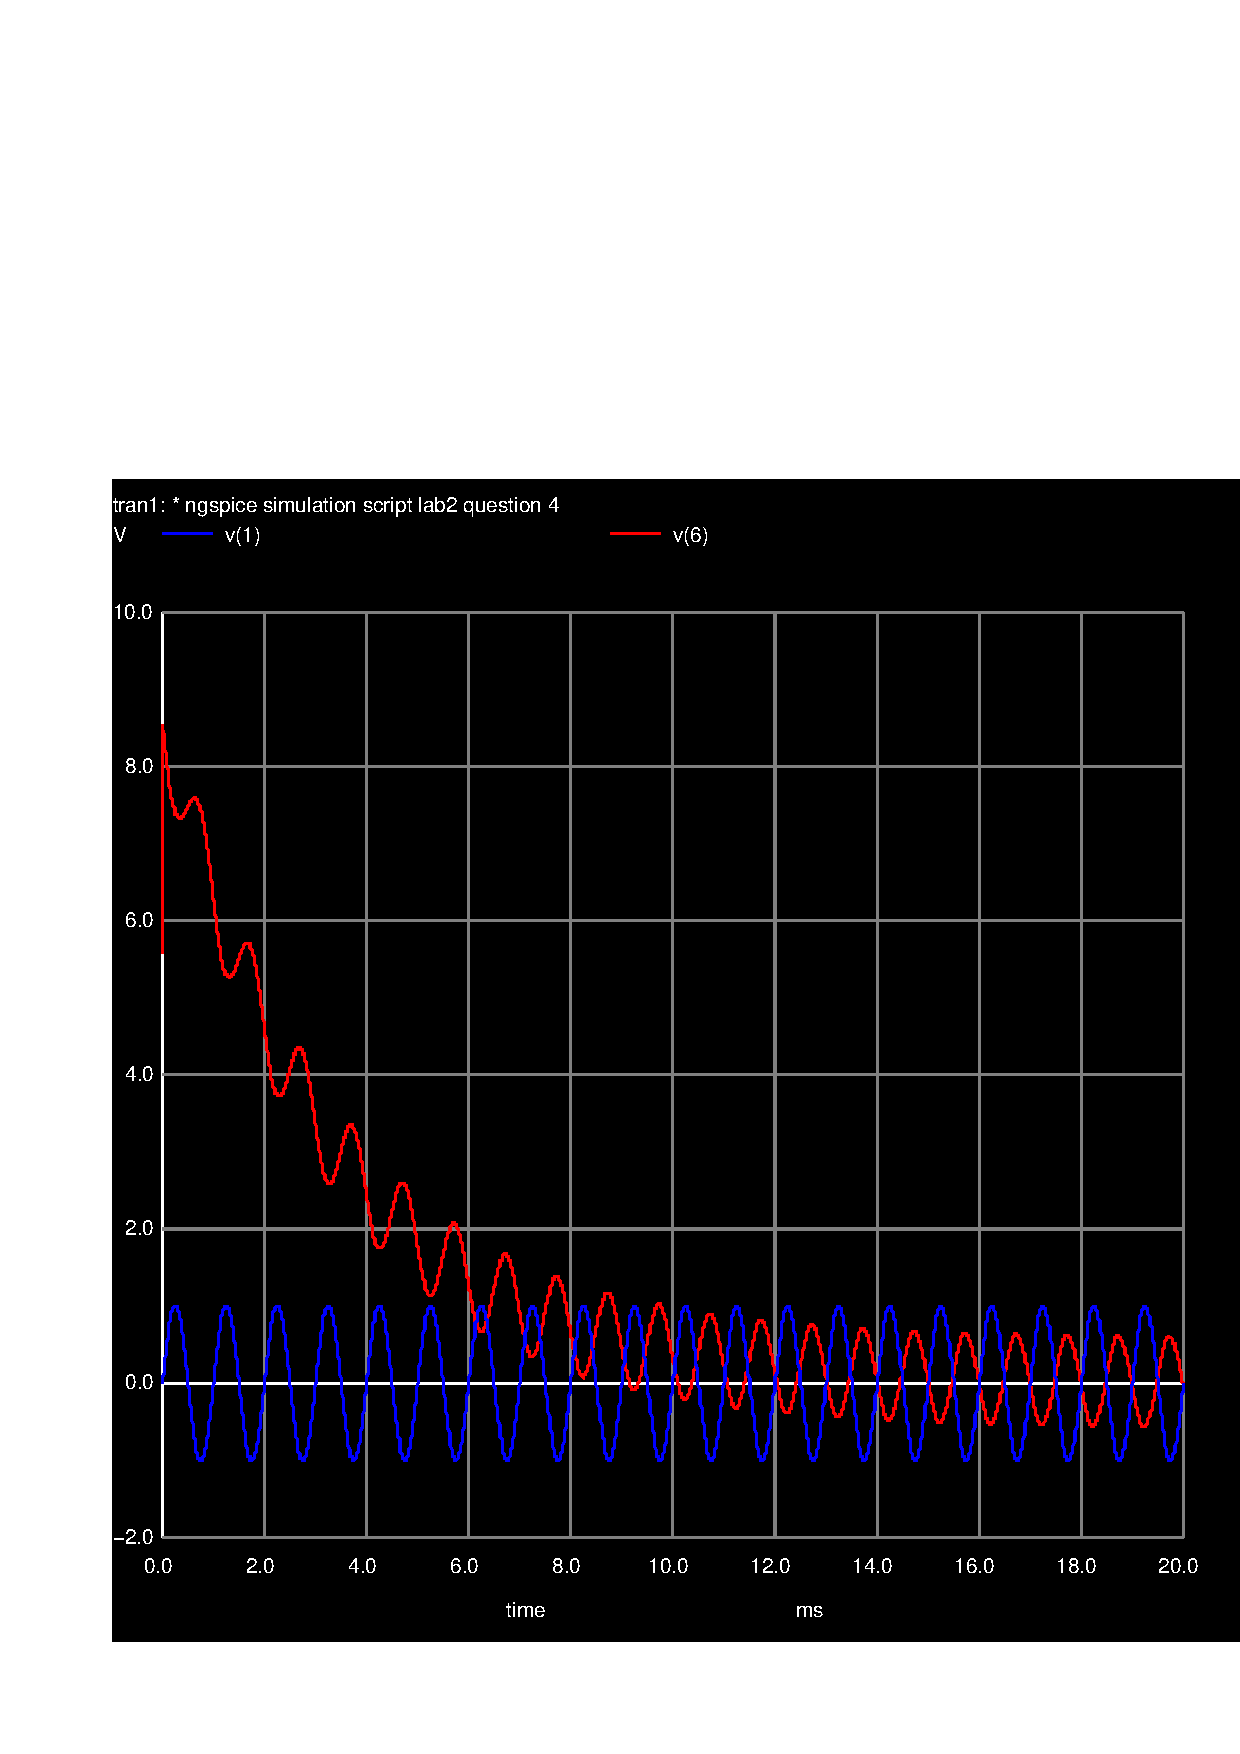
\includegraphics[width=0.4\linewidth]{sim4.pdf}
\caption{Total Response - Ngspice}
\label{fig:sim4}
\end{figure}

\subsection{Comparison}
 When observing \ref{fig:sim4}, we conclude that, in the period of time considered, the voltage in the capacitor tends to diminuish until its phase differs $\pi$ from the phase of the voltage source. The same result has also been accomplish in the theoretical analysis, as seen in \ref{fig:part4}.

\newpage


\subsection{Frequency Responses}



In this part of the assignment, an AC (Small Signal Analysis was conducted, in order to match the goal aforementioned. This type of analysis allows to study the frequency response of the circuit. In other words, there is no frequency variation over time, the so called steady-state analysis.


\subsubsection{Frequency Response- Magnitude}

\begin{figure}[h] \centering
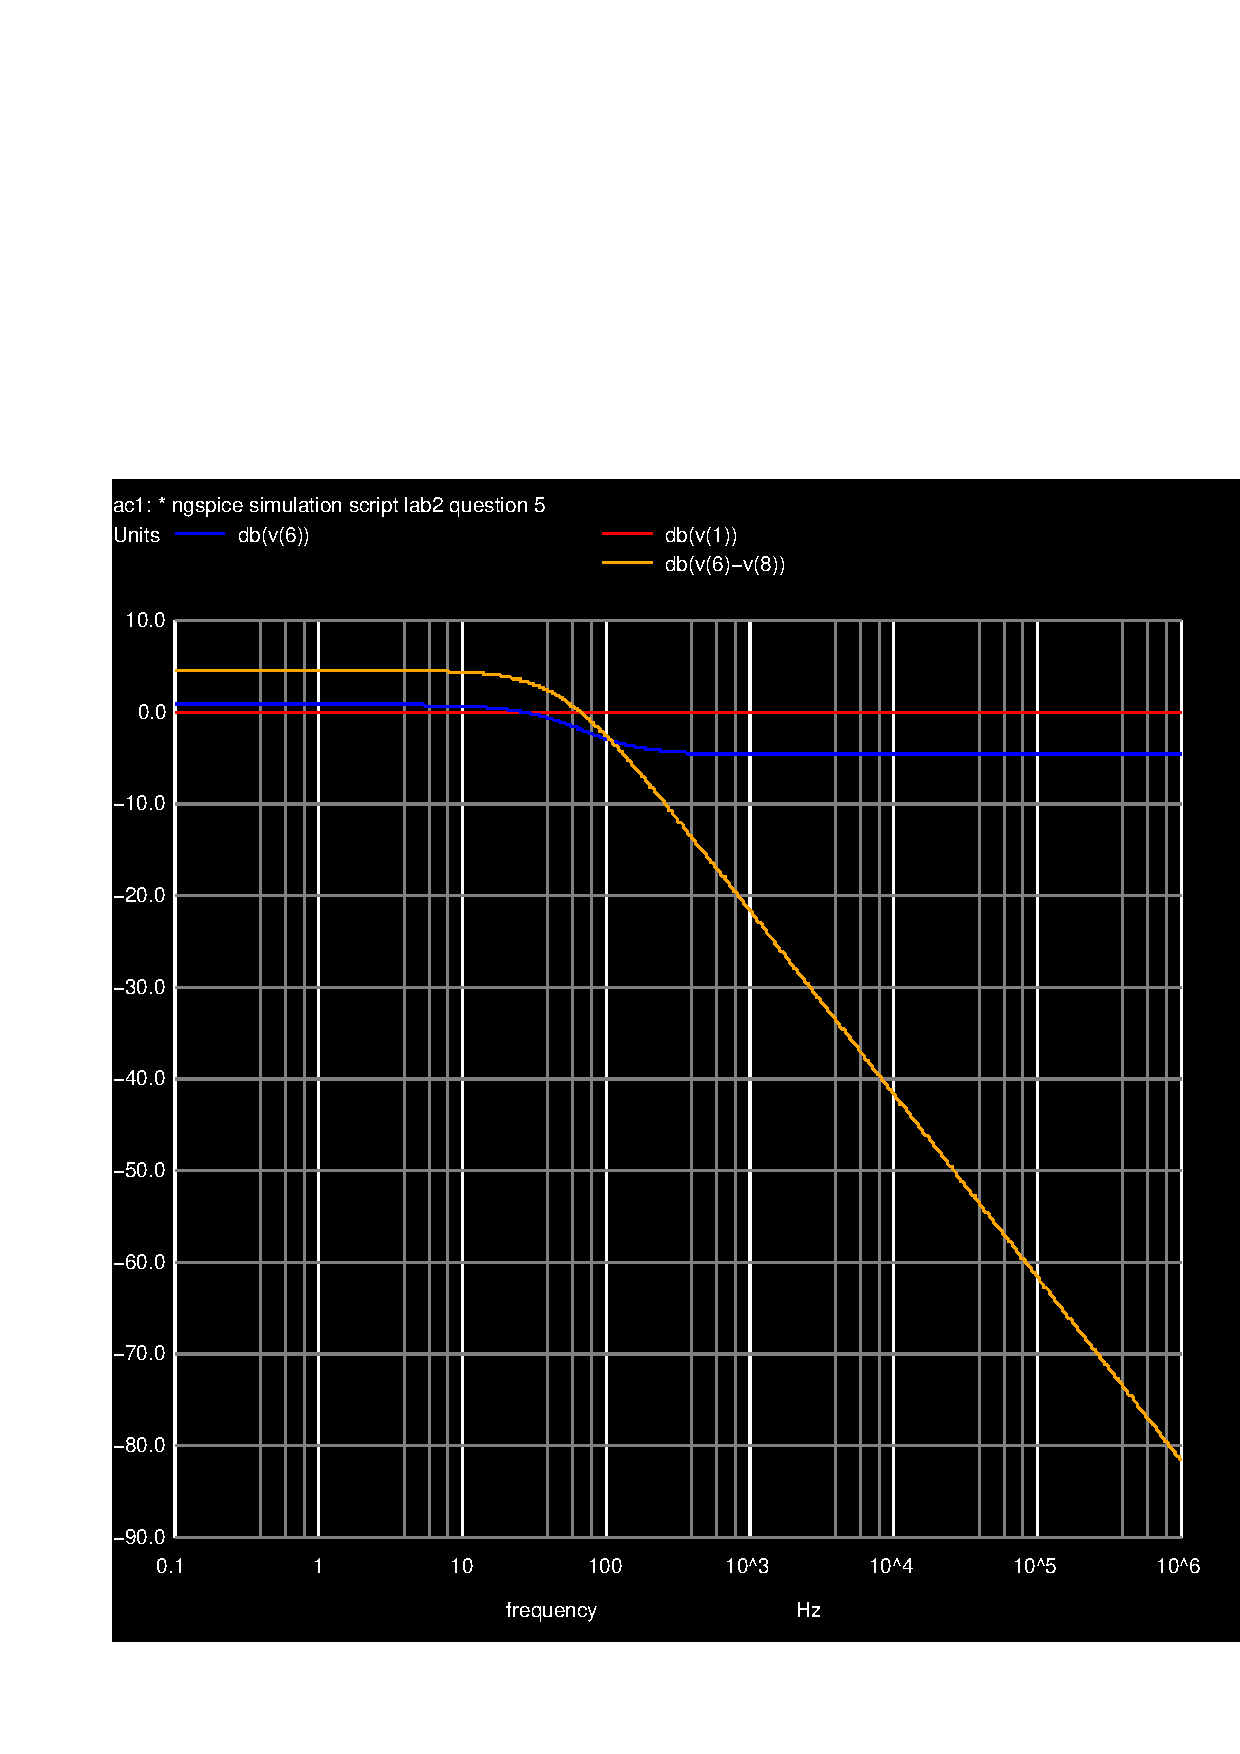
\includegraphics[width=0.4\linewidth]{sim5_db.pdf}
\caption{Magnitude Response (in decibels)}
\label{fig:sim5_db}
\end{figure}

\subsubsection{Frequency Response- Phase}


\begin{figure}[h] \centering
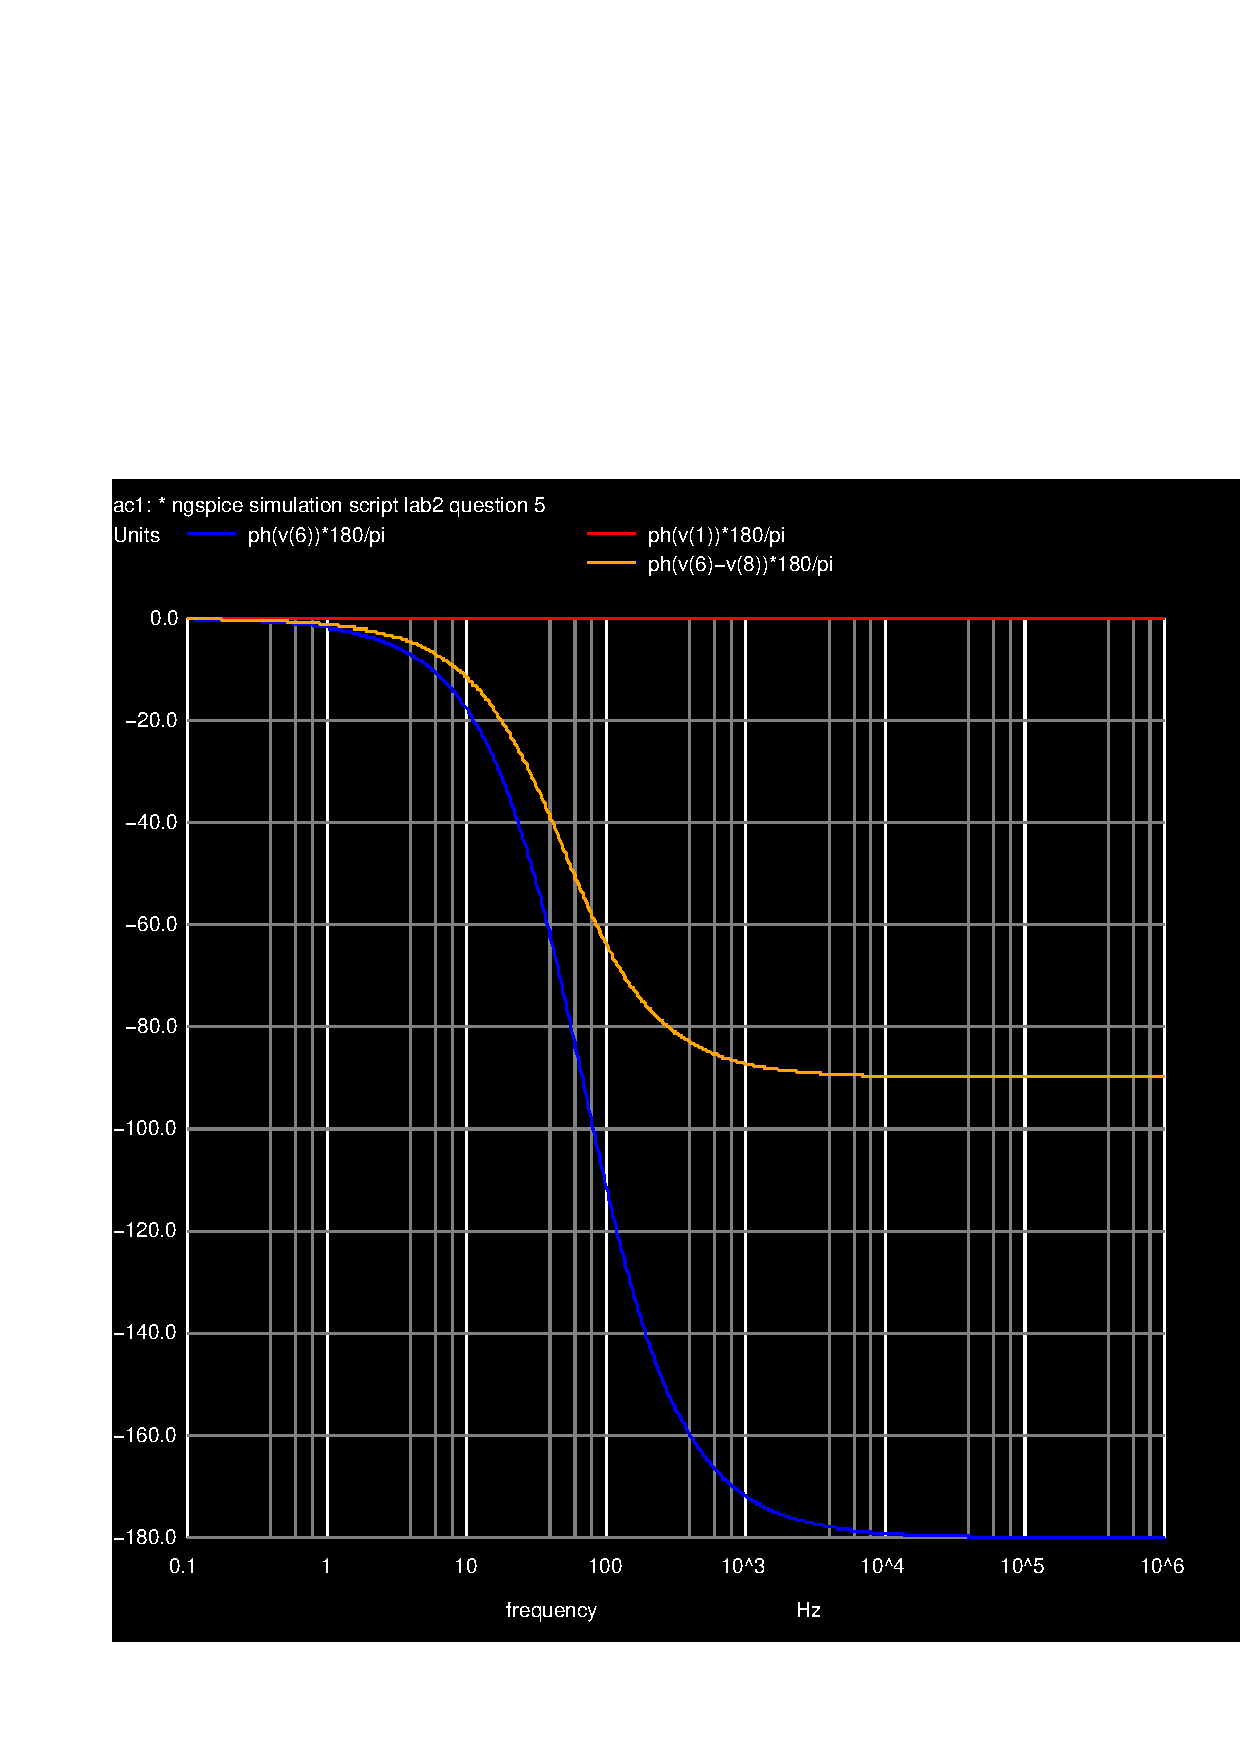
\includegraphics[width=0.4\linewidth]{sim5_ph.pdf}
\caption{Phase Response (in degrees)}
\label{fig:sim5_ph}
\end{figure}
\newpage

After comparing the graphics showed below, it is clear to admit that the results in ngspice and octave match. Any minor difference may be explained by aproximation errors.




